\section{Elementary Astronomy}

\begin{multicols}{2}


\section*{The Solar System}


\subsection{Student Solar System}

\begin{center}
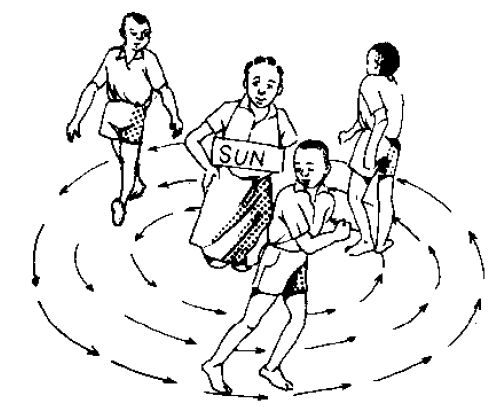
\includegraphics[width=0.4\textwidth]{./img/source/student-solar-system.png}
\end{center}

\begin{description*}
%\item[Subtopic:]{}
\item[Materials:]{}
\item[Setup:]{}
\item[Procedure:]{}
\item[Hazards:]{}
\item[Questions:]{}
\item[Observations:]{}
\item[Theory:]{}
\item[Applications:]{}
\item[Notes:]{}
\end{description*}

\subsection{Solar System Mobile}

%\begin{center}
%\includegraphics[width=0.4\textwidth]{./img/source/.png}
%\end{center}

\begin{description*}
%\item[Subtopic:]{}
\item[Materials:]{}
\item[Setup:]{}
\item[Procedure:]{}
\item[Hazards:]{}
\item[Questions:]{}
\item[Observations:]{}
\item[Theory:]{}
\item[Applications:]{}
\item[Notes:]{}
\end{description*}

%==================================================================================================%

\section*{Gravitational Force}


\subsection{Centripetal Force}

\begin{center}
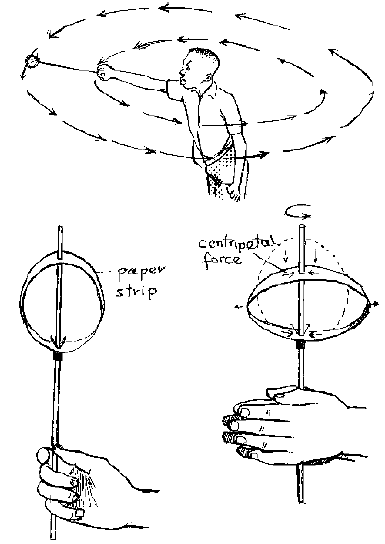
\includegraphics[width=0.4\textwidth]{./img/source/centripetal-force.png}
\end{center}

\begin{description*}
%\item[Subtopic:]{}
\item[Materials:]{}
\item[Setup:]{}
\item[Procedure:]{}
\item[Hazards:]{}
\item[Questions:]{}
\item[Observations:]{}
\item[Theory:]{}
\item[Applications:]{}
\item[Notes:]{}
\end{description*}

\subsection{Bucket Swing}

\begin{center}
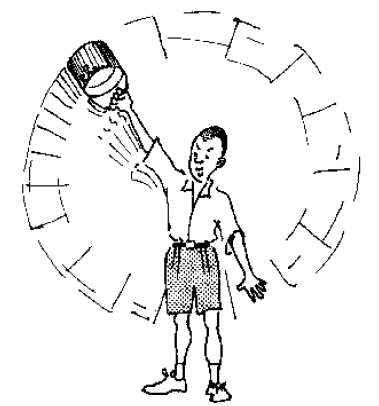
\includegraphics[width=0.4\textwidth]{./img/source/bucket-swing.png}
\end{center}

\begin{description*}
%\item[Subtopic:]{}
\item[Materials:]{}
\item[Setup:]{}
\item[Procedure:]{}
\item[Hazards:]{}
\item[Questions:]{}
\item[Observations:]{}
\item[Theory:]{}
\item[Applications:]{}
\item[Notes:]{}
\end{description*}

%==================================================================================================%

\section*{Constellations}


\subsection{Star Gazing}

%\begin{center}
%\includegraphics[width=0.4\textwidth]{./img/source/.png}
%\end{center}

\begin{description*}
%\item[Subtopic:]{}
\item[Materials:]{}
\item[Setup:]{}
\item[Procedure:]{}
\item[Hazards:]{}
\item[Questions:]{}
\item[Observations:]{}
\item[Theory:]{}
\item[Applications:]{}
\item[Notes:]{}
\end{description*}

%==================================================================================================%

\section*{The Earth and Its Moon}


\subsection{Model of Sun-Earth-Moon}

\begin{center}
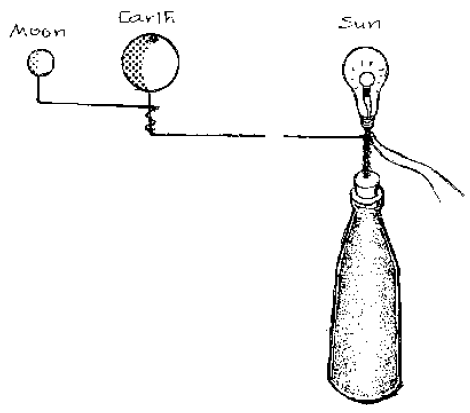
\includegraphics[width=0.4\textwidth]{./img/source/sun-earth-moon.png}
\end{center}

\begin{description*}
%\item[Subtopic:]{}
\item[Materials:]{}
\item[Setup:]{}
\item[Procedure:]{}
\item[Hazards:]{}
\item[Questions:]{}
\item[Observations:]{}
\item[Theory:]{}
\item[Applications:]{}
\item[Notes:]{}
\end{description*}

%==================================================================================================%



\end{multicols}

\pagebreak